An op amp having a low-frequency gain of $10^{3}$ and a single-pole rolloff at $10^{4}$ rad/s is connected in a negative feedback loop via a feedback network having a transmission k and a two-pole rolloff at $10^{4}$ rad/s. Find the value of k above which the closed-loop amplifier becomes unstable.
\begin{enumerate}[label=\arabic*.,ref=\theenumi]

%\begin{enumerate}[label=\thesection.\arabic*.,ref=\thesection.\theenumi]
\numberwithin{equation}{enumi}

\item Find the OPAMP gain $G(s)$
\\
\solution 
The given oscillator has a low frequency gain $10^3$ and a single-pole rolloff at $10^4$ rad/s. So we have a open loop amplifier gain 
\begin{align}
G(s)&= \frac{10^3}{1+\frac{s}{10^4}}
\end{align}
\item Find the feedback $H(s)$
\\
\solution 
\begin{align}
H(s)&= \frac{k}{\left(1+\frac{s}{10^4}\right)^2}   
\end{align}
%
\item Find the  loop-gain. 
\\
\solution The loop gain is given by 
\begin{align}
L(s) = G(s)H(s) &= \frac{10^3k}{\left(1+\frac{s}{10^4}\right)^3}
\end{align}
and the various gains summarised in Table \ref{table:ee18btech11006_Factors}

\begin{table}[!ht]
\centering
\input{./tables/ee18btech11006/ee18btech11006_1.tex}
\caption{}
\label{table:ee18btech11006_Factors}
\end{table}
%\\
%The closed loop gain would be
%\begin{align}
%T(s)=\frac{G(s)}{1+G(s)H(s)}
%\end{align}
%Generalized condition for the system to be stable:
%\begin{align}
%T(j\omega)=\frac{G(j\omega)}{1+G(j\omega)H(j\omega)}
%\end{align}
%Loop gain, $L(j\omega)=G(j\omega)H(j\omega)$.
%\begin{align}
%L(j\omega)=\abs{{G(j\omega)H(j\omega)}}e^{j\phi(\omega)}
%\end{align}
%Let 
%\begin{align}
%\exp\cbrak{\j \phase{L\brak{\j \omega_{\pi}}}} = -1
%\end{align}
%Let the frequency at which phase angle $\phi(\omega)$ becomes $180^{\circ}$ be $\omega_{180}$. At $\omega = \omega_{180}$ , $L(j\omega)$ is a negative real number.
\item Find the condition for stability.
\\
\solution 
For stability, $\left(GM\right)_{dB} \And PM > 0$. \\
%\begin{itemize}
%    \item if $\abs{{G(j\omega_{180})H(j\omega_{180})}}$ $<$ 1,$T(j\omega_{180}) >$ 1 \\ $\implies$ 
%    system is stable.
%    \item if $\abs{{G(j\omega_{180})H(j\omega_{180})}}$ $=$ 1,$T(j\omega_{180}) = \infty $ \\ $\implies$
%    system is unstable.
%    \item if $\abs{{G(j\omega_{180})H(j\omega_{180})}}$ $>$ 1,$T(j\omega_{180}) <$ 1 \\ $\implies$ 
%    system is unstable.
%\end{itemize}
For the given system :
\begin{align}
   \angle G(j\omega)H(j\omega) =  \angle\frac{10^3k}{\left(1+\frac{j\omega}{10^4}\right)^3} 
   = -3tan^{-1}\left({\frac{\omega}{10^4}}\right)
\end{align}
So the phase crossover frequency is,
\begin{align}
   180^{\circ}= \abs{-3tan^{-1}\left({\frac{\omega_{180}}{10^4}}\right)}\\
   \implies \omega_{180} = \sqrt{3}\times 10^4
\end{align}
The Loop gain at $\omega_{180}$ is $\abs{G(j\omega_{180})H(j\omega_{180})}$.
 (i) $GM_{dB} > 0$
\begin{align}
\implies \abs{G(j\omega_{180})H(j\omega_{180})}< 1 \\
\implies \abs{\frac{10^3k}{\left(1+\frac{j\omega}{10^4}\right)^3}} < 1\\
\abs{\frac{10^3k}{\left(1-\sqrt{3}j\right)^3} } < 1
\end{align}
\begin{align}
     \frac{10^3\abs{k}}{{\abs{\sqrt{1+{\sqrt{3}}^2}}}^3} < 1\\
     \frac{10^3\abs{k}}{8} < 1 \\
     \implies \abs{k} < 0.008
\end{align}
(ii) $PM=\phi_m=180^{\circ}+\angle{L\left(j\omega_{gc}\right)}>0 $ i.e..   $180^{\circ}-3tan^{-1}\left({\frac{\omega_{gc}}{10^4}}\right)>0$.\\
Gain crossover frequency $\omega_{gc}$,
\begin{align}
   \abs{G(j\omega_{gc})H(j\omega_{gc})}= 1  \\
   \abs{\frac{10^3k}{{\sqrt{1+\frac{{\omega_{gc}}^2}{10^8}}}^3}}=1\\
  \implies \omega_{gc}=\sqrt{10^8\left(10^2k^{\frac{2}{3}}-1\right)}
\end{align}
Now, 
\begin{align}
  \phi_m=180^{\circ}-3tan^{-1}\left({\frac{\sqrt{10^8\left(10^2k^{\frac{2}{3}}-1\right)}}{10^4}}\right)>0  
\end{align}
\begin{align}
\sqrt{10^8\left(10^2k^{\frac{2}{3}}-1\right)}&<\sqrt{3} \times 10^4\\
10^2k^{\frac{2}{3}}&<4\\
\implies \abs{k}<0.008
\end{align}
From (i) and (ii) the value of k above which the system becomes unstable is 0.008.
\item Design the feedback circuit $H$. \\
\solution
\begin{align}
H(s)&=\frac{V_f}{V_0}= \frac{k}{\left(1+\frac{s}{10^4}\right)^2} = k\left({\frac{1}{1+\frac{2s}{10^4}+\frac{s^2}{10^8}}}\right)  
\end{align}
This is of the form,
\begin{align}
k\left(\frac{1}{1+s{R_1}{C_1}+{s^2}{L_1}{C_1}}\right) =  k\left(\frac{\frac{1}{s{C_1}}}{{R_1}+s{L_1}+\frac{1}{s{C_1}}}\right)  
\end{align}
This can be realized using the circuit,
\begin{figure}[!ht]
	\begin{center}
		\resizebox{\columnwidth}{!}{\begin{circuitikz}
\ctikzset{bipoles/length=1cm}

\draw 
(0, 0) node[op amp] (opamp) {}
(opamp.-) -- (-2,0.35)  node[ground]{}
(opamp.out) to[L =$L_1$,*-*] (2,0)to[R=$R_1$](4,0) to [C](4,-2.4) node[ground]{}
(opamp.+)   to (-1.8,-0.35)node at (-2,-0.35){$V_0$}
(opamp.center) node[]{k};
\draw node at (4.6,-1.2){$V_f$}
node at (4.6,0){$+$}
node at (4.6,-2.4){$-$}
node at (3.5,-1.2){$C_1$}
;\end{circuitikz}
}
	\end{center}
\caption{}
\label{fig:ee18btech11006_2}
\end{figure} \\
A set of values that satisfy these equations are,
\begin{align}
R_1&= 200\ohm \\
C_1&= 1\mu F\\
L_1&= 10mH 
\end{align}
\item Design the closed loop circuit.  You may choose a suitable vale of $k$ such that the system is stable.\\
\solution Let k=0.001. The closed loop gain is T(s).
\begin{align}
    T(s)&=\frac{\frac{10^3}{1+\frac{s}{10^4}}}{1+\frac{1}{\left(1+\frac{s}{10^4}\right)^3}}\\
    &=\frac{10^7s^2+2\times10^{11}s+10^{15}}{s^3+3\times10^4s^2+3\times10^8s+2\times10^{12}}
\end{align}
The final circuit would be:
\begin{figure}[!ht]
	\begin{center}
		\resizebox{\columnwidth}{!}{\input{./figs/ee18btech11006/ee18btech11006_6.tex}}
	\end{center}
\caption{}
\label{fig:ee18btech11006_6}
\end{figure}
\begin{align}
R_1&= 200\ohm \\
C_1&= 1\mu F\\
L_1&= 10mH \\
L_2&=1\mu F\\
R_2&=100\ohm\\
k&=10^{-3}
\end{align}
\item Sketch the Bode plot of the closed loop system
\solution The following code gives the Bode plot of the closed loop system
\begin{lstlisting}
codes/ee18btech11006/ee18btech11006_1.py
\end{lstlisting}
Bode Plot:
\begin{figure}[ht!]
\centering
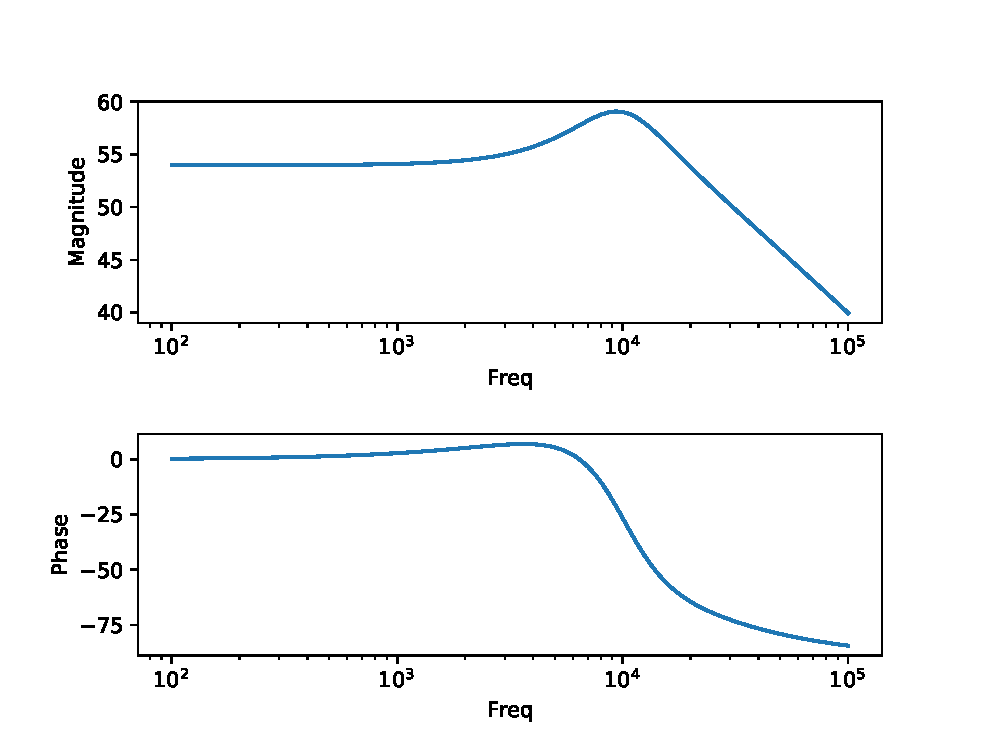
\includegraphics[width=\columnwidth]{./figs/ee18btech11006/ee18btech11006_7.eps}
\caption{}
\label{fig:ee18btech11006_7}
\end{figure}
\item Find the output of the circuit for an appropriate input using spice.\\
\solution
The following readme file provides necessary instructions to simulate the circuit in spice.
\begin{lstlisting}
codes/ee18btech11006/spice/README
\end{lstlisting}
The following netlist simulates the given circuit.
\begin{lstlisting}
codes/ee18btech11006/spice/ee18btech11006.net
\end{lstlisting}
The following code plots the output from the spice simulation which is shown in Fig. \ref{fig:ee18btech11006_8}.
\begin{lstlisting}
codes/ee18btech11006/spice/ee18btech11006_spice.py
\end{lstlisting}
\renewcommand{\thefigure}{\theenumi.\arabic{figure}}
%
\begin{figure}[!ht]
\centering
\includegraphics[width=\columnwidth]{./figs/ee18btech11006/ee18btech11006_8.eps}
\caption{}
\label{fig:ee18btech11006_8}
\end{figure}
\textbf{Verification}: The Output of the system would be :
\begin{align}
    Y(s)&=T(s)X(s)\\
    X(s)&=\frac{A}{s}\\
    Y(s)&=A\frac{10^7s^2+2\times10^{11}s+10^{15}}{s^4+3\times10^4s^3+3\times10^8s^2+2\times10^{12}s}
\end{align}
The following python codes plot the inverse Laplace of Y(s) giving the time domain output for different values of A.
\begin{lstlisting}
codes/ee18btech11006/spice/ee18btech11006_2.py
\end{lstlisting}
On plotting, we obtain the given figure.\\
\begin{figure}[!ht]
\centering
\includegraphics[width=\columnwidth]{./figs/ee18btech11006/ee18btech11006_9.eps}
\caption{}
\label{fig:ee18btech11006_9}
\end{figure}
Hence verified that the designed circuit does represent the given system.
\end{enumerate}

